% !TeX spellcheck = en_GB
\begin{figure}[t]
	\centering
    \begin{subfigure}[b]{0.49\textwidth}
    	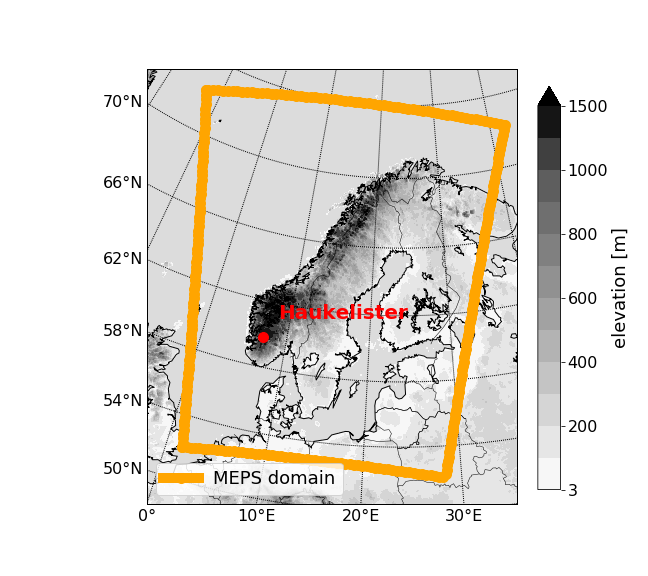
\includegraphics[trim={2.75cm 1.8cm 4.4cm 2.3cm},clip,
        width=\textwidth]{./fig_Norway/Norway_MEPS}
        \caption{}\label{fig:site:Norway}
    \end{subfigure}
 %%%%% zoomed in map
    \begin{subfigure}[b]{0.49\textwidth}
    	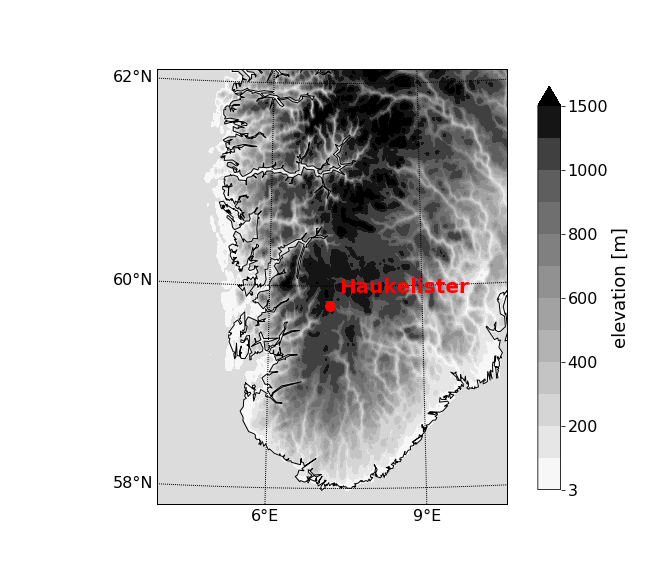
\includegraphics[trim={2.75cm 1.8cm .65cm 2.3cm},clip,
        width=\textwidth]{./fig_Norway/South_Norway}
    	\caption{}\label{fig:site:Nzoom}
    \end{subfigure}
   	\caption{Elevation map of Northern Europe and South Norway, \subref{fig:site:Norway}, \subref{fig:site:Nzoom} respectively. Red dot indicates the location Haukeliseter and the orange square in \subref{fig:site:Norway} indicates the model domain of MEPS. Elevation according to the shading.} \label{fig:site}
\end{figure}